\documentclass{article}
\usepackage{amsmath}
\usepackage{tikz}
\usepackage{hyperref}
\usetikzlibrary{chains,fit,shapes}

\author{Andrew McIsaac}
\title{Introduction to Complexity and Computability: Homework 1}
\date{\today}


\begin{document}
\maketitle

\subsection*{Homework Problem 1}
%Show that any single-tape Turing machine \textit{M} can be converted to a Turing
%machine \textit{M'} which is allowed to execute only two of the three actions at
%one step, that is, any instruction either
%\begin{itemize}
%	\item changes state and head position, or
%	\item changes state and tape symbol, or
%	\item changes head position and tape symbol,
%\end{itemize}
%but no instruction can perform all three of these actions.

A single-tape Turing machine $M$ can be converted to a TM $M'$ by
modifying the transition function so that any single transition performed by
$M$ is performed in two transitions by $M'$.

The first transition changes the state and tape symbol to the desired tape
symbol and the intermediate state consists of a tuple with the desired state and
desired head position. The second transition then changes state and head
position based on the state and head position stored in the state of the
intermediate transition.

The set of states of $M'$, $Q'$, is augmented, so that $Q' = Q \cup Q \times \{L,R\}$

E.g. For $M$, a transition $\delta{(q, a)} = (q', a', L)$ is done in $M'$ with
two steps:
\begin{align*}
	\delta{(q,a)} &= ((q', L), a') \\
	\delta{((q', L), a')} &= (q', L)
\end{align*}	

\subsection*{Homework Problem 2}
%Consider a Turing machine model where the tape is
%only one-way infinite (to the right) and the head can only perform two types of
%movement: right (R) or RESTART (that is, return to the first field of the tape).
%Show how to convert a single-tape Turing machine to a Turing machine of this kind.

A single-tape TM $M$ can be converted to a TM $M'$ where the tape is one-way
infinite with only right (R) and RESTART head movements by creating $M'$ where
the head movements of $M$ are replicated in the following way.

For R movements from $M$, $M'$ exactly replicates the movement of $M$.

For L movements from $M$, $M'$ first marks the current tape symbol, then
performs a RESTART movement. The head then proceeds right, entirely replicating
the input tape one step to the right, with the first symbol being replaced
by a placeholder symbol. This continues until the marked symbol is reached,
where the tape symbol to the left of the original marked symbol is marked in its
place, and the rest of the input then continues to be copied, unmarking the
originally marked symbol. Finally, the tape is RESTARTed, and moves right until
the marked symbol is reached.

This marked symbol can perform exactly the same transitions as the unmarked
symbol, and is overwritten by either the unmarked symbol or a new symbol
depending on the next transition (or is kept marked if the next transition is a
left transition, restarting the process described above). The head is
effectively  one position left of its original position, with the entire
original tape shifted one position to the right. Fig. \ref{fig:tape} shows an
example diagram of this notion.

\begin{figure}
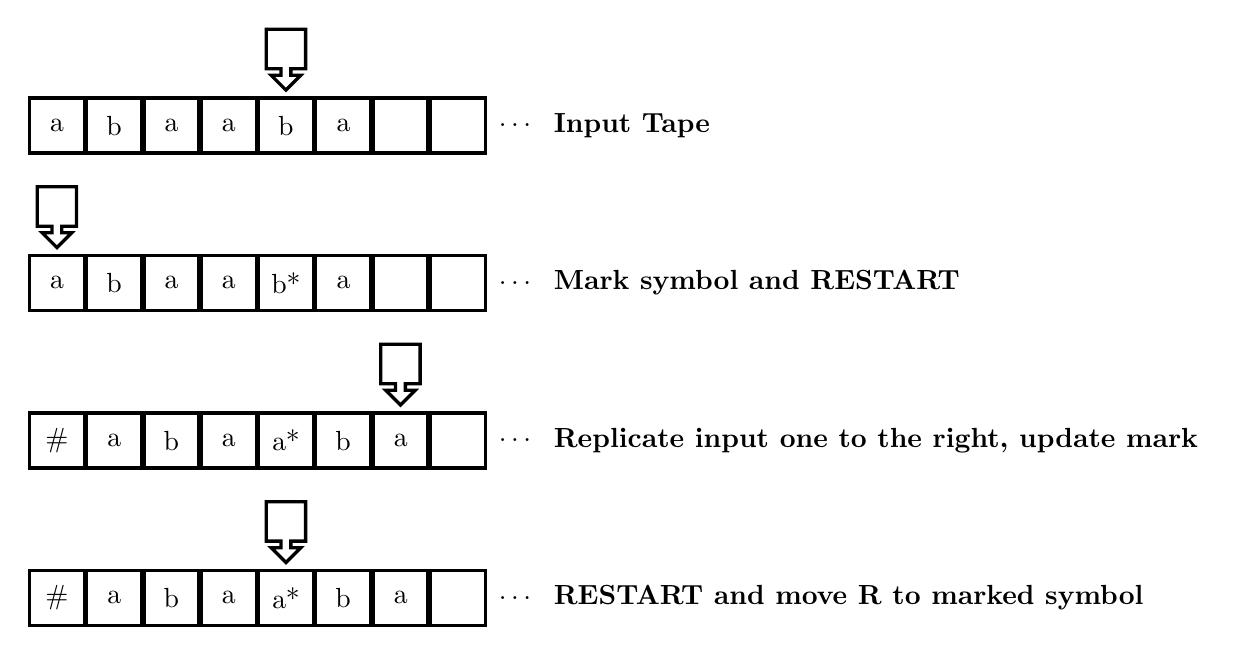
\begin{tikzpicture}
\tikzstyle{every path}=[very thick]

\edef\sizetape{0.7cm}
\tikzstyle{tmtape}=[draw,minimum size=\sizetape]
\tikzstyle{tmhead}=[arrow box,draw,minimum size=.5cm,arrow box
arrows={east:.25cm, west:0.25cm}]
\tikzstyle{tmheadpos}=[arrow box,draw,minimum size=.5cm,arrow box
arrows={south:.25cm}]

%% Draw TM tape
\begin{scope}[shift={(0cm,0cm)},start chain=1 going right,node distance=-0.15mm]
    \node [on chain=1,tmtape] {a};
    \node [on chain=1,tmtape] {b};
    \node [on chain=1,tmtape] {a};
    \node [on chain=1,tmtape] {a};
    \node [on chain=1,tmtape] (head) {b};
	\node [on chain=1,tmtape] {a};
    \node [on chain=1,tmtape] {};
    \node [on chain=1,tmtape] {};
    \node [on chain=1,tmtape,draw=none] {$\ldots$};
    \node [on chain=1] {\textbf{Input Tape}};
\end{scope}

%% Draw TM head below (input) tape cell
\node [tmheadpos,yshift=0.6cm] at (head.north) (head) {};

%% Draw TM tape
\begin{scope}[shift={(0cm,-2cm)},start chain=1 going right,node distance=-0.15mm]
    \node [on chain=1,tmtape] (head) {a};
    \node [on chain=1,tmtape] {b};
    \node [on chain=1,tmtape] {a};
    \node [on chain=1,tmtape] {a};
	\node [on chain=1,tmtape] {b*};
	\node [on chain=1,tmtape] {a};
    \node [on chain=1,tmtape] {};
    \node [on chain=1,tmtape] {};
    \node [on chain=1,tmtape,draw=none] {$\ldots$};
    \node [on chain=1] {\textbf{Mark symbol and RESTART}};
\end{scope}

%% Draw TM head below (input) tape cell
\node [tmheadpos,yshift=0.6cm] at (head.north) (head) {};

%% Draw TM tape
\begin{scope}[shift={(0cm,-4cm)},start chain=1 going right,node distance=-0.15mm]
    \node [on chain=1,tmtape] {\#};
    \node [on chain=1,tmtape] {a};
    \node [on chain=1,tmtape] {b};
    \node [on chain=1,tmtape] {a};
    \node [on chain=1,tmtape] {a*};
	\node [on chain=1,tmtape] {b};
	\node [on chain=1,tmtape] (head) {a};
    \node [on chain=1,tmtape] {};
    \node [on chain=1,tmtape,draw=none] {$\ldots$};
	\node [on chain=1] {\textbf{Replicate input one to the right, update mark}};
\end{scope}

%% Draw TM head below (input) tape cell
\node [tmheadpos,yshift=0.6cm] at (head.north) (head) {};

%% Draw TM tape
\begin{scope}[shift={(0cm,-6cm)},start chain=1 going right,node distance=-0.15mm]
    \node [on chain=1,tmtape] {\#};
    \node [on chain=1,tmtape] {a};
    \node [on chain=1,tmtape] {b};
    \node [on chain=1,tmtape] {a};
	\node [on chain=1,tmtape] (head) {a*};
	\node [on chain=1,tmtape] {b};
	\node [on chain=1,tmtape] {a};
    \node [on chain=1,tmtape] {};
    \node [on chain=1,tmtape,draw=none] {$\ldots$};
    \node [on chain=1] {\textbf{RESTART and move R to marked symbol}};
\end{scope}

%% Draw TM head below (input) tape cell
\node [tmheadpos,yshift=0.6cm] at (head.north) (head) {};
\end{tikzpicture}
\caption{TM $M'$ simulating effective left movement of TM $M$. The result shows
the entire original input tape replicated on the same tape but one cell to the
right, with the head position in its original place.}
\label{fig:tape}
\end{figure}

\end{document}
